\chapter{Multiparty secure computation II: Construction using Fully
Homomorphic Encryption}\label{sfetwochap}

In the last lecture we saw the definition of secure multiparty
computation, as well as the compiler reducing the task of achieving
security in the general (malicious) setting to the passive
(honest-but-curious) setting. In this lecture we will see how using
fully homomorphic encryption we can achieve security in the
honest-but-curious setting.\footnote{This is by no means the only way to
  get multiparty secure computation. In fact, multiparty secure
  computation was known well before FHE was discovered. One common
  construction for achieving this uses a technique known as \emph{Yao's
  Garbled Circuit}.} We focus on the two party case, and so prove the
following theorem:

\hypertarget{twopartympc}{}
\begin{theorem}[Two party honest-but-curious MPC] \label[theorem]{twopartympc}

Assuming the LWE conjecture, for every two party functionality \(F\)
there is a protocol computing \(F\) in the honest but curious model.

\end{theorem}

Before proving the theorem it might be worthwhile to recall what is
actually the definition of secure multiparty computation, when
specialized for the \(k=2\) and honest but curious case. The definition
significantly simplifies here since we don't have to deal with the
possibility of aborts.

\hypertarget{twopartympcdef}{}
\begin{definition}[Two party honest-but-curious secure computation] \label[definition]{twopartympcdef}

Let \(F\) be (possibly probabilistic) map of
\(\{0,1\}^n\times \{0,1\}^n\) to \(\{0,1\}^n\times\{0,1\}^n\). A
\emph{secure protocol for \(F\)} is a two party protocol such for every
party \(t\in \{1,2\}\), there exists an efficient ``ideal adversary''
(i.e., efficient interactive algorithm) \(S\) such that for every pair
of inputs \((x_1,x_2)\) the following two distributions are
computationally indistinguishable:

\begin{itemize}
\item
  The tuple \((y_1,y_2,v)\) obtained by running the protocol on inputs
  \(x_1,x_2\), and letting \(y_1,y_2\) be the outputs of the two parties
  and \(v\) be the \emph{view} (all internal randomness, inputs, and
  messages received) of party \(t\).
\item
  The tuple \((y_1,y_2,v)\) that is computed by letting
  \((y_1,y_2)=F(x_1,x_2)\) and \(v=S(x_t,y_t)\).
\end{itemize}

That is, \(S\), which only gets the input \(x_t\) and output \(y_t\),
can simulate all the information that an honest-but-curious adversary
controlling party \(t\) will view.

\end{definition}

\section{Constructing 2 party honest but curious computation from fully
homomorphic encryption}\label{17-Constructing--party-ho}

Let \(F\) be a two party functionality. Lets start with the case that
\(F\) is \emph{deterministic} and that only Alice receives an output.
We'll later show an easy reduction from the general case to this one.
Here is a suggested protocol for Alice and Bob to run on inputs \(x,y\)
respectively so that Alice will learn \(F(x,y)\) but nothing more about
\(y\), and Bob will learn nothing about \(x\) that he didn't know
before.

\begin{marginfigure}
\centering
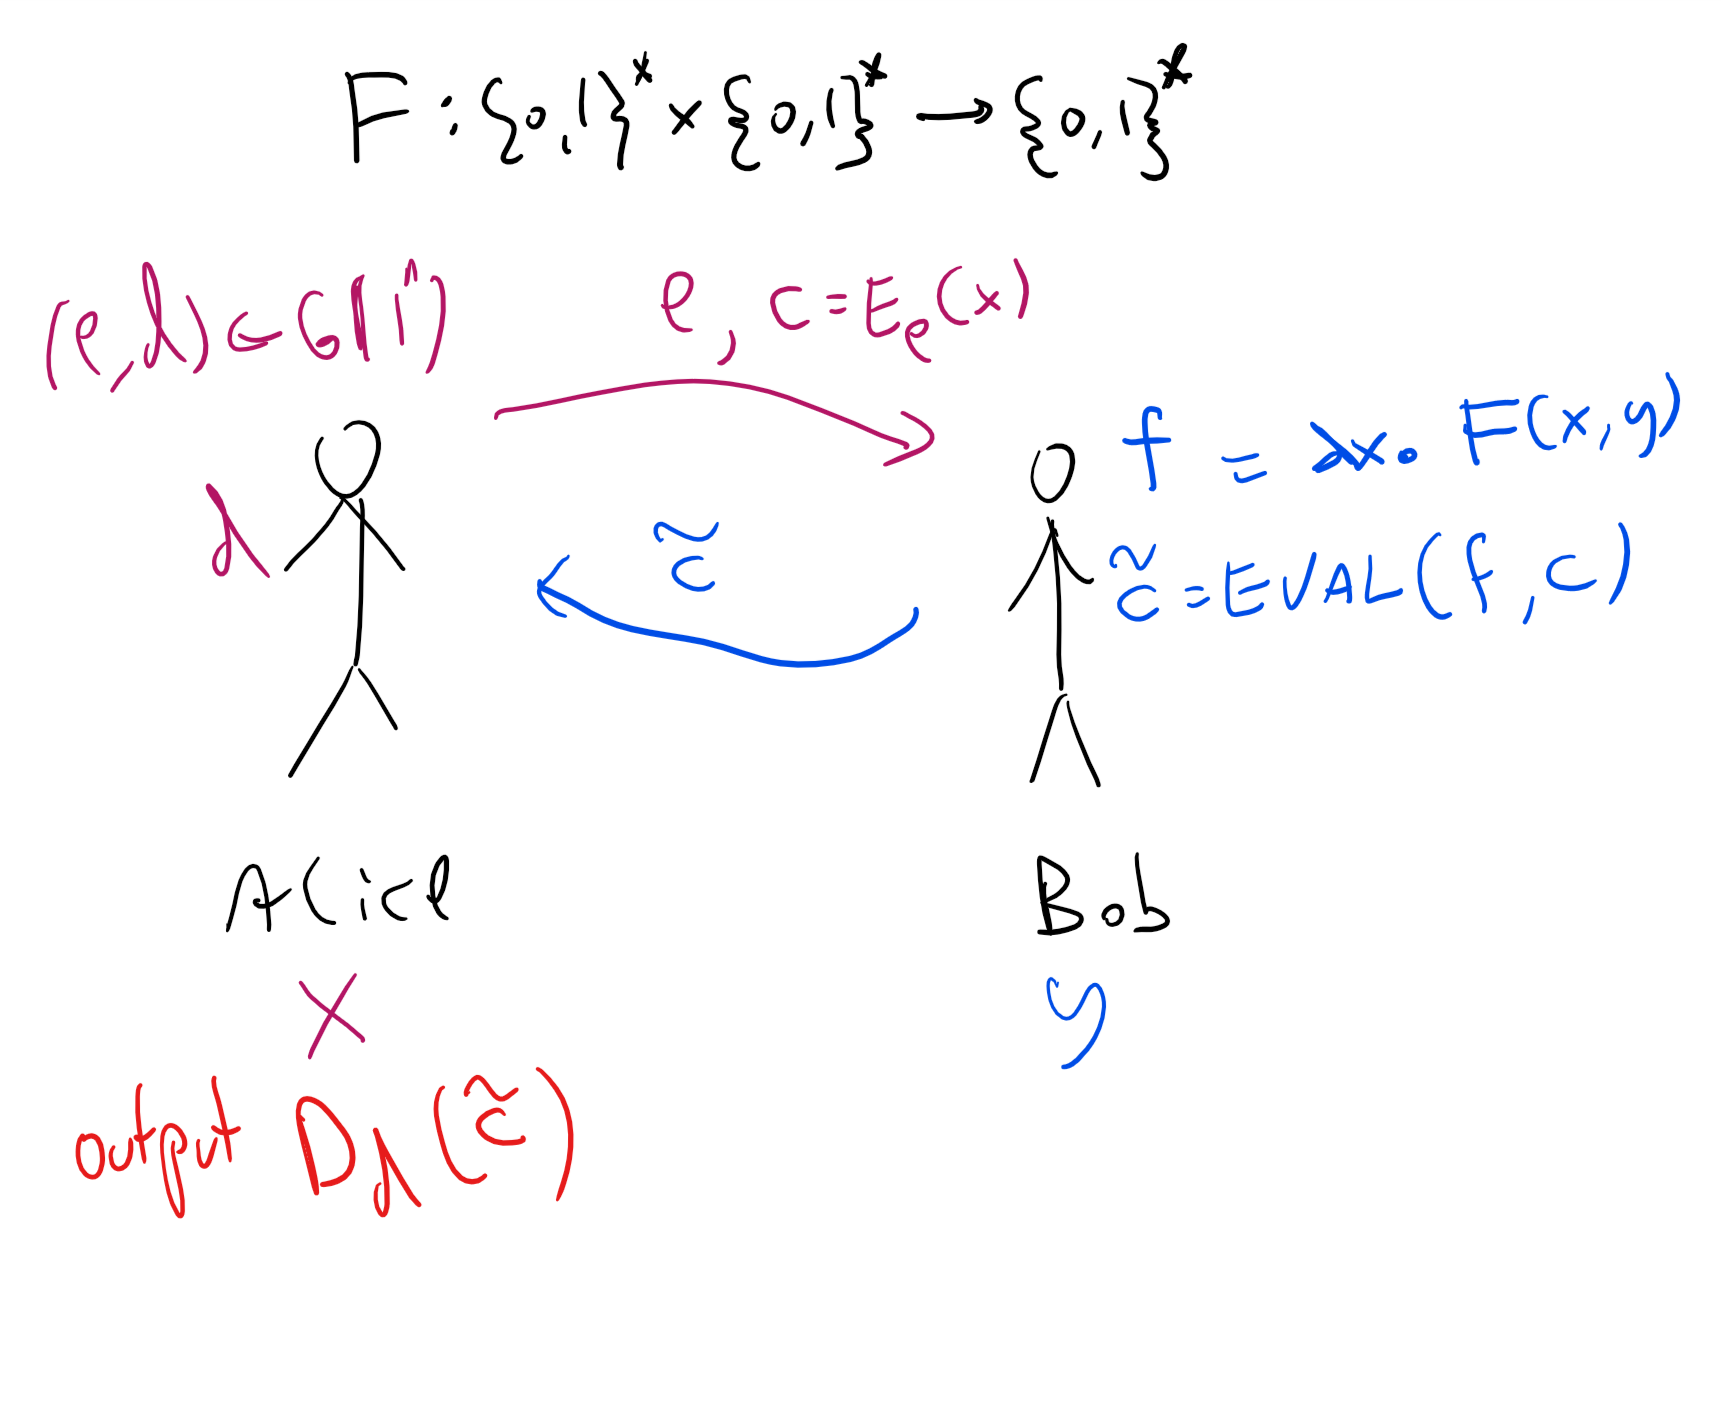
\includegraphics[width=\linewidth, height=1.5in, keepaspectratio]{../figure/twopcprotfig.png}
\caption{An honest but curious protocol for two party computation using
a fully homomorphic encryption scheme with circuit privacy.}
\label{twopcprotfig}
\end{marginfigure}

::: \textbf{Protocol 2PC:} (See \cref{twopcprotfig})

\begin{itemize}
\item
  \textbf{Assumptions:} \((G,E,D,\ensuremath{\mathit{EVAL}})\) is a
  fully homomorphic encryption scheme.
\item
  \textbf{Inputs:} Alice's input is \(x\in\{0,1\}^n\) and Bob's input is
  \(y\in\{0,1\}^n\). The goal is for Alice to learn only \(F(x,y)\) and
  Bob to learn nothing.
\item
  \textbf{Alice-\textgreater Bob:} Alice generates
  \((e,d)\leftarrow_R G(1^n)\) and sends \(e\) and \(c=E_e(x)\).
\item
  \textbf{Bob-\textgreater Alice:} Bob computes define \(f\) to be the
  function \(f(x)=F(x,y)\) and sends
  \(c'=\ensuremath{\mathit{EVAL}}(f,c)\) to Alice.
\item
  \textbf{Alice's output:} Alice computes \(z=D_d(c')\).
\end{itemize}

:::

First, note that if Alice and Bob both follow the protocol, then indeed
at the end of the protocol Alice will compute \(F(x,y)\). We now claim
that Bob does not learn anything about Alice's input:

\paragraph{Claim B:} For every \(x,y\), there exists a standalone
algorithm \(S\) such that \(S(y)\) is indistinguishable from Bob's view
when interacting with Alice and their corresponding inputs are
\((x,y)\).

\paragraph{Proof:} Bob only receives a single message in this protocol
of the form \((e,c)\) where \(e\) is a public key and \(c=E_e(x)\). The
simulator \(S\) will generate \((e,d) \leftarrow_R G(1^n)\) and compute
\((e,c)\) where \(c=E_e(0^n)\). (As usual \(0^n\) denotes the length
\(n\) string consisting of all zeroes.) No matter what \(x\) is, the
output of \(S\) is indistinguishable from the message Bob receives by
the security of the encryption scheme. QED

(In fact, Claim B holds even against a \emph{malicious} strategy of Bob-
can you see why?)

We would now hope that we can prove the same regarding Alice's security.
That is prove the following:

\paragraph{Claim A:} For every \(x,y\), there exists a standalone
algorithm \(S\) such that \(S(y)\) is indistinguishable from Alice's
view when interacting with Bob and their corresponding inputs are
\((x,y)\).

\begin{pause} \label[pause]{17-At-this-point-you-migh}

At this point, you might want to try to see if you can prove Claim A on
your own. If you're having difficulties proving it, try to think whether
it's even true.

\end{pause}

.

.

.

.

.

.

.

.

.

.

\newpage

So, it turns out that Claim A is \emph{not} generically true. The reason
is the following: the definition of fully homomorphic encryption only
requires that \(\ensuremath{\mathit{EVAL}}(f,E(x))\) decrypts to
\(f(x)\) but it does \emph{not} require that it hides the contents of
\(f\). For example, for every FHE, if we modify
\(\ensuremath{\mathit{EVAL}}(f,c)\) to append to the ciphertext the
first \(100\) bits of the description of \(f\) (and have the decryption
algorithm ignore this extra information) then this would still be a
secure FHE.\footnote{It's true that strictly speaking, we allowed
  \(\ensuremath{\mathit{EVAL}}\)'s output to have length at most \(n\),
  while this would make the output be \(n+100\), but this is just a
  technicality that can be easily bypassed, for example by having a new
  scheme that on security parameter \(n\) runs the original scheme with
  parameter \(n/2\) (and hence will have a lot of ``room'' to pad the
  output of \(\ensuremath{\mathit{EVAL}}\) with extra bits).} Now we
didn't exactly specify how we describe the function \(f(x)\) defined as
\(x \mapsto F(x,y)\) but there are clearly representations in which the
first \(100\) bits of the description would reveal the first few bits of
the hardwired constant \(y\), hence meaning that Alice will learn those
bits from Bob's message.

Thus we need to get a stronger property, known as \emph{circuit
privacy}. This is a property that's useful in other contexts where we
use FHE. Let us now define it:

\hypertarget{perfectcircprivatedef}{}
\begin{definition}[Perfect circuit privacy] \label[definition]{perfectcircprivatedef}

Let \(\mathcal{E}=(G,E,D,\ensuremath{\mathit{EVAL}})\) be an FHE. We say
that \(\mathcal{E}\) satisfies \emph{perfect circuit privacy} if for
every \((e,d)\) output by \(G(1^n)\) and every function
\(f:\{0,1\}^\ell\rightarrow\{0,1\}\) of \(poly(n)\) description size,
and every ciphertexts \(c_1,\ldots,c_\ell\) and
\(x_1,\ldots,x_\ell \in \{0,1\}\) such that \(c_i\) is output by
\(E_e(x_i)\), the distribution of
\(\ensuremath{\mathit{EVAL}}_e(f,c_1,\ldots,c_\ell)\) is identical to
the distribution of \(E_e(f(x))\). That is, for every \(z\in\{0,1\}^*\),
the probability that
\(\ensuremath{\mathit{EVAL}}_e(f,c_1,\ldots,c_\ell)=z\) is the same as
the probability that \(E_e(f(x))=z\). We stress that these probabilities
are taken only over the coins of the algorithms
\(\ensuremath{\mathit{EVAL}}\) and \(E\).

\end{definition}

Perfect circuit privacy is a strong property, that also automatically
implies that
\(D_d(\ensuremath{\mathit{EVAL}}(f,E_e(x_1),\ldots,E_e(x_\ell)))=f(x)\)
(can you see why?). In particular, once you understand the definition,
the following lemma is a fairly straightforward exercise.

\hypertarget{circprivacylem}{}
\begin{lemma} \label[lemma]{circprivacylem}

If \((G,E,D,\ensuremath{\mathit{EVAL}})\) satisfies perfect circuit
privacy then if \((e,d) = G(1^n)\) then for every two functions
\(f,f':\{0,1\}^\ell\rightarrow\{0,1\}\) of \(poly(n)\) description size
and every \(x\in\{0,1\}^\ell\) such that \(f(x)=f'(x)\), and every
algorithm \(A\),
\[| \Pr[ A(d,\ensuremath{\mathit{EVAL}}(f,E_e(x_1),\ldots,E_e(x_\ell)))=1] -  \Pr[ A(d,\ensuremath{\mathit{EVAL}}(f',E_e(x_1),\ldots,E_e(x_\ell)))=1] | < negl(n) \label{eqcircprivacy}.\]

\end{lemma}

\begin{pause} \label[pause]{17-Please-stop-here-and-t}

Please stop here and try to prove \cref{circprivacylem}

\end{pause}

The algorithm \(A\) above gets the \emph{secret key} as input, but still
cannot distinguish whether the \(\ensuremath{\mathit{EVAL}}\) algorithm
used \(f\) or \(f'\). In fact, the expression on the lefthand side of
\eqref{eqcircprivacy} is equal to \emph{zero} when the scheme satisfies
perfect circuit privacy.\\
However, for our applications bounding it by a negligible function is
enough. Hence, we can use the relaxed notion of ``imperfect'' circuit
privacy, defined as follows:

\hypertarget{circprivatedef}{}
\begin{definition}[Statistical circuit privacy] \label[definition]{circprivatedef}

Let \(\mathcal{E}=(G,E,D,\ensuremath{\mathit{EVAL}})\) be an FHE. We say
that \(\mathcal{E}\) satisfies \emph{statistical circuit privacy} if for
every \((e,d)\) output by \(G(1^n)\) and every function
\(f:\{0,1\}^\ell\rightarrow\{0,1\}\) of \(poly(n)\) description size,
and every ciphertexts \(c_1,\ldots,c_\ell\) and
\(x_1,\ldots,x_\ell \in \{0,1\}\) such that \(c_i\) is output by
\(E_e(x_i)\), the distribution of
\(\ensuremath{\mathit{EVAL}}_e(f,c_1,\ldots,c_\ell)\) is equal up to
\(negl(n)\) total variation distance to the distribution of
\(E_e(f(x))\).

That is,
\begin{equation*}
\sum_{z\in\{0,1\}^*} \left| \Pr[ \ensuremath{\mathit{EVAL}}_e(f,c_1,\ldots,c_\ell)=z] - \Pr[ E_e(f(x))=z ] \right| < negl(n)
\end{equation*}

where once again, these probabilities are taken only over the coins of
the algorithms \(\ensuremath{\mathit{EVAL}}\) and \(E\).

\end{definition}

If you find \cref{circprivatedef} hard to parse, the most important
points you need to remember about it are the following:

\begin{itemize}
\item
  Statistical circuit privacy is as good as perfect circuit privacy for
  all applications, and so you can imagine the latter notion when using
  it.
\item
  Statistical circuit privacy can easier to achieve in constructions.
\end{itemize}

(The third point, which goes without saying, is that you can always ask
clarifying questions in class, Piazza, sections, or office hours\ldots)

Intuitively, circuit privacy corresponds to what we need in the above
protocol to protect Bob's security and ensure that Alice doesn't get any
information about his input that she shouldn't have from the output of
\(\ensuremath{\mathit{EVAL}}\), but before working this out, let us see
how we can construct fully homomorphic encryption schemes satisfying
this property.

\section{Achieving circuit privacy in a fully homomorphic
encryption}\label{17-Achieving-circuit-priv}

We now discuss how we can modify our fully homomorphic encryption
schemes to achieve the notion of circuit privacy. In the scheme we saw,
the encryption of a bit \(b\), whether obtained through the encryption
algorithm or \(\ensuremath{\mathit{EVAL}}\), always had the form of a
matrix \(C\) over \(\Z_q\) (for \(q=2^{\sqrt{n}}\)) where
\(Cv = bv + e\) for some vector \(e\) that is ``small'' (e.g., for every
\(i\), \(|e_i| < n^{polylog(n)}\ll q=2^{\sqrt{n}}\)). However, the
\(\ensuremath{\mathit{EVAL}}\) algorithm was \emph{deterministic} and
hence this vector \(e\) is a function of whatever function \(f\) we are
evaluating and someone that knows the secret key \(v\) could recover
\(e\) and then obtain from it some information about \(f\). We want to
make \(\ensuremath{\mathit{EVAL}}\) probabilistic and lose that
information, and we use the following approach

\begin{quote}
\emph{To kill a signal, drown it in lots of noise}
\end{quote}

That is, if we manage to add some additional random noise \(e'\) that
has magnitude much larger than \(e\), then it would essentially
``erase'' any structure \(e\) had. More formally, we will use the
following lemma:

\hypertarget{noiseandsignallem}{}
\begin{lemma} \label[lemma]{noiseandsignallem}

Let \(a\in \Z_q\) and \(T\in\mathbb{N}\) be such that \(aT<q/2\). If we
let \(X\) be the distribution obtained by taking \(x (\mod q)\) for an
integer \(x\) chosen at random in \([-T,+T]\) and let \(X'\) be the
distribution obtained by taking \(a+x (\mod q)\) for \(x\) chosen in the
same way, then
\begin{equation*}
\sum_{y \in \Z_q} \left| \Pr[X=y] - \Pr[X'=y] \right| <|a|/T
\end{equation*}

\end{lemma}

\begin{marginfigure}
\centering
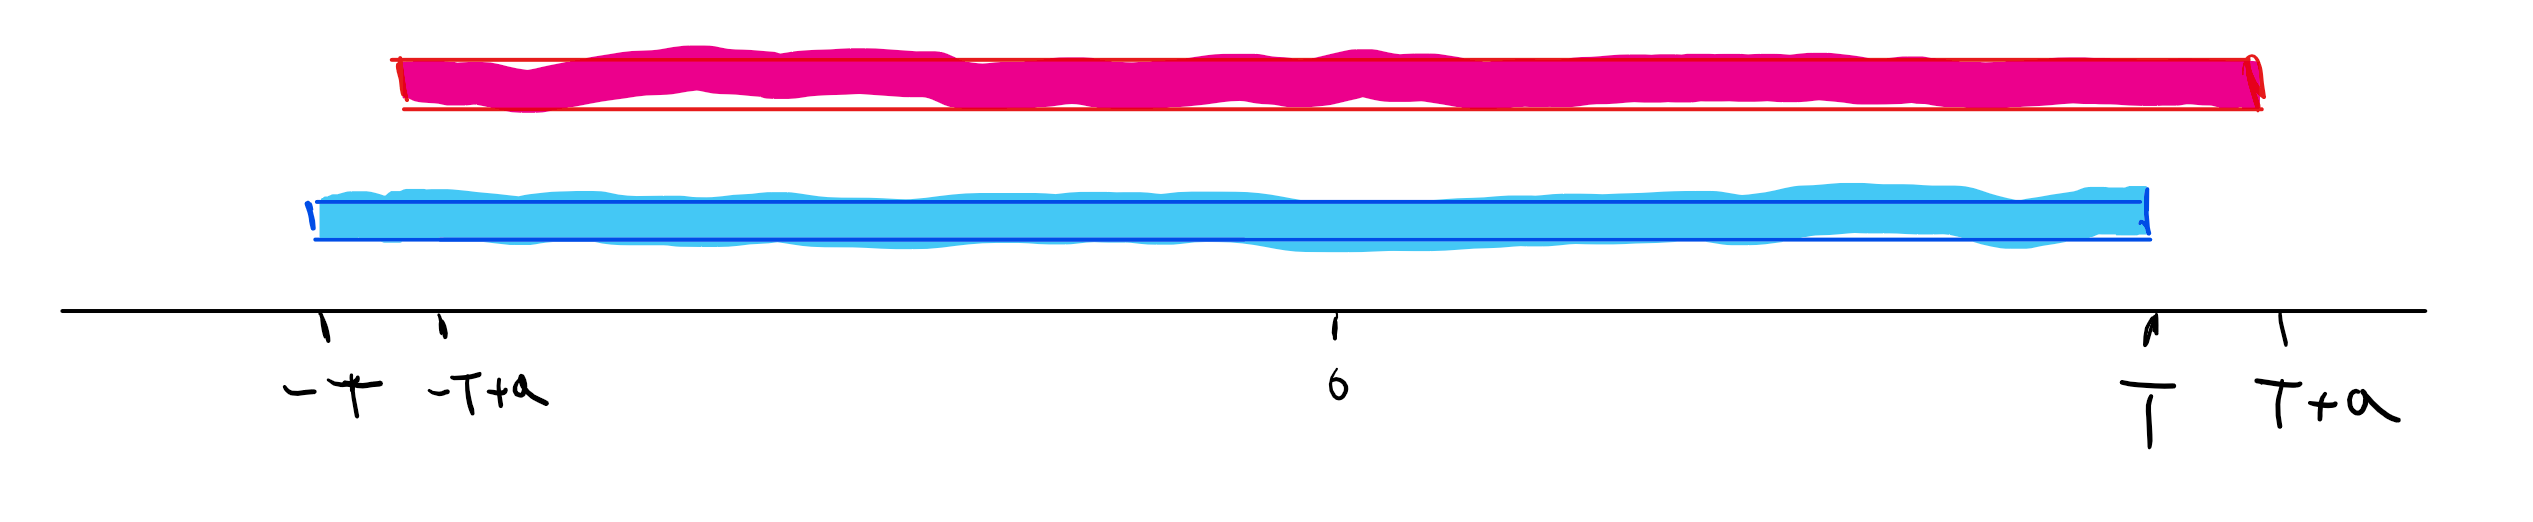
\includegraphics[width=\linewidth, height=1.5in, keepaspectratio]{../figure/statdistintervals.png}
\caption{If \(a \ll T\) then the uniform distribution over the interval
\([-T,+T]\) is statistically close to the uniform distribution over the
interval \([-T+a,+T+a]\), since the statistical distance is proportional
to the event (which happens with probability \(a/T\)) that a random
sample from one distribution falls inside the symmetric difference of
the two intervals.}
\label{statdistintervalsfig}
\end{marginfigure}

\begin{proof} \label[proof]{17-This-has-a-simple-proo}

This has a simple ``proof by picture'': consider the intervals
\([-T,+T]\) and \([-T+a,+T+a]\) on the number line (see
\cref{statdistintervalsfig}). Note that the symmetric difference of
these two intervals is only about a \(a/T\) fraction of their union.
More formally, \(X\) is the uniform distribution over the \(2T+1\)
numbers in the interval \([-T,+T]\) while \(X'\) is the uniform
distribution over the shifted version of this interval \([-T+a,+T+a]\).
There are exactly \(2|a|\) numbers which get probability zero under one
of those distributions and probability \((2T+1)^{-1}<(2T)^{-1}\) under
the other.

\end{proof}

We will also use the following lemma:

\hypertarget{productstatisticialdistlem}{}
\begin{lemma} \label[lemma]{productstatisticialdistlem}

If two distributions over numbers \(X\) and \(X'\) satisfy
\(\Delta(X,X')=\sum_{y\in\Z}|\Pr[X=x]-\Pr[Y=y]|<\delta\) then the
distributions \(X^m\) and \(X'^m\) over \(m\) dimensional vectors where
every entry is sampled independently from \(X\) or \(X'\) respectively
satisfy \(\Delta(X^m,X'^m) \leq m\delta\).

\end{lemma}

\begin{pause} \label[pause]{17-We-omit-the-proof-of-c}

We omit the proof of \cref{productstatisticialdistlem} and leave it as
an exercise to prove it using the hybrid argument. We will actually only
use \cref{productstatisticialdistlem} for distributions above; you can
obtain intuition for it by considering the \(m=2\) case where we compare
the rectangles of the forms \([-T,+T]\times [-T,+T]\) and
\([-T+a,+T+a]\times[-T+b,+T+b]\). You can see that their union has size
roughly \(4T^2\) while their symmetric difference has size roughly
\(2T\cdot 2a + 2T\cdot 2b\), and so if \(|a|,|b| \leq \delta T\) then
the symmetric difference is roughly a \(2\delta\) fraction of the union.

\end{pause}

We will not provide the full details, but together these lemmas show
that \(\ensuremath{\mathit{EVAL}}\) can use bootstrapping to reduce the
magnitude of the noise to roughly \(2^{n^{0.1}}\) and then add an
additional random noise of roughly, say, \(2^{n^{0.2}}\) which would
make it statistically indistinguishable from the actual encryption. Here
are some hints on how to make this work: the idea is that in order to
``re-randomize'' a ciphertext \(C\) we need a very noisy encryption of
zero and add it to \(C\). The normal encryption will use noise of
magnitude \(2^{n^{0.2}}\) but we will provide an encryption of the
secret key with smaller magnitude \(2^{n^{0.1}/polylog(n)}\) so we can
use bootstrapping to reduce the noise. The main idea that allows to add
noise is that at the end of the day, our scheme boils down to LWE
instances that have the form \((c,\sigma)\) where \(c\) is a random
vector in \(\Z_q^{n-1}\) and \(\sigma = \langle c,s \rangle+a\) where
\(a \in [-\eta,+\eta]\) is a small noise addition. If we take any such
input and add to \(\sigma\) some \(a' \in [-\eta',+\eta']\) then we
create the effect of completely re-randomizing the noise. However,
completely analyzing this requires non-trivial amount of care and work.

\subsection{Bottom line: A two party secure computation
protocol}\label{17-Bottom-line-A-two-part}

Using the above we can obtain the following theorem:

\hypertarget{rerandfhethm}{}
\begin{theorem}[Re-randomizable FHE] \label[theorem]{rerandfhethm}

If the LWE conjecture is true then there exists a tuple of
polynomial-time randomized algorithms
\((G,E,D,\ensuremath{\mathit{EVAL}},\ensuremath{\mathit{RERAND}})\) such
that:

\begin{itemize}
\item
  \((G,E,D,\ensuremath{\mathit{EVAL}})\) is a CPA secure
  fully-homomorphic encryption for one bit messages. That is, if
  \((d,e)=G(1^n)\) then for every Boolean circuit \(C\) with \(\ell\)
  inputs and one output, and \(x\in \{0,1\}^\ell\), the ciphertext
  \(c = \ensuremath{\mathit{EVAL}}_e(C, E_e(x_1),\ldots, E_e(x_\ell)\)
  has length \(n\) and \(D_d(c)=C(x)\) with probability one over the
  random choices of the algorithms \(E\) and
  \(\ensuremath{\mathit{EVAL}}\).
\item
  For every pair of keys \((e,d) =G(1^n)\) there are two distributions
  \(\mathcal{C}^0,\mathcal{C}^1\) over \(\{0,1\}^n\) such that:

  \begin{itemize}
  \item
    For \(b\in \{0,1\}\),
    \(\Pr_{c \sim \mathcal{C}^b} [ D_d(c) = b ]=1\). That is,
    \(\mathcal{C}^b\) is distributed over ciphertexts that decrypt to
    \(b\).
  \item
    For every ciphertext \(c \in \{0,1\}^n\) in the image of either
    \(E_e(\cdot)\) or \(\ensuremath{\mathit{EVAL}}_e(\cdot)\), if
    \(D_d(c)=b\) then \(\ensuremath{\mathit{RERAND}}_e(c)\) is
    statistically indistinguishable from \(\mathcal{C}^b\). That is, the
    output of \(\ensuremath{\mathit{RERAND}}_e(c)\) is a ciphertext that
    decrypts to the same plaintext as \(c\), but whose distribution is
    essentially independent of \(c\).
  \end{itemize}
\end{itemize}

\end{theorem}

\begin{proofidea} \label[proofidea]{17-We-do-not-include-the-}

We do not include the full proof but the idea is we use our standard
LWE-based FHE and to rerandomize a ciphertext \(c\) we will add to it an
encryption of \(0\) (which will not change the corresponding plaintext)
and an additional noise vector that would be of much larger magnitude
than the original noise vector of \(c\), but still small enough so
decryption succeeds.

\end{proofidea}

Using the above re-randomizable encryption scheme, we can redefine
\(\ensuremath{\mathit{EVAL}}\) to add a \(\ensuremath{\mathit{RERAND}}\)
step at the end and achieve statistical circuit privacy. If we use
Protocol 2PC with such a scheme then we get a two party computation
protocol secure with respect to honest but curious adversaries. Using
the compiler of \cref{hbctomalthm} we obtain a proof of \cref{MPCthm}
for the two party setting:

\hypertarget{twopartycthm}{}
\begin{theorem}[Two party secure computation] \label[theorem]{twopartycthm}

If the LWE conjecture is true then for every (potentially randomized)
functionality
\(F:\{0,1\}^{n_1} \times \{0,1\}^{n_2} \rightarrow \{0,1\}^{m_1} \times \{0,1\}^{m_2}\)
there exists a polynomial-time protocol for computing the functionality
\(F\) secure with respect to potentially \emph{malicious} adversaries.

\end{theorem}

\section{Beyond two parties}\label{17-Beyond-two-parties}

We now sketch how to go beyond two parties. It turns out that the
compiler of honest-but-curious to malicious security works just as well
in the many party setting, and so the crux of the matter is to obtain an
\emph{honest but curious} secure protocol for \(k>2\) parties.

We start with the case of three parties - Alice, Bob, and Charlie.
First, let us introduce some convenient notation (which is used in other
settings as well).\footnote{I believe this notation originates with
  Burrows--Abadi--Needham (BAN) logic though would be happy if scribe
  writers verify this.} We will assume that each party initially
generates private/public key pairs with respect to some fully
homomorphic encryption (satisfying statistical circuit privacy) and
sends them to the other parties. We will use \(\{ x \}_A\) to denote the
encryption of \(x\in \{0,1\}^\ell\) using Alice's public key (similarly
\(\{ x \}_B\) and \(\{ x \}_C\) will denote the encryptions of \(x\)
with respect to Bob's and Charlie's public key. We can also compose
these and so denote by \(\{ \{ x \}_A \}_B\) the encryption under Bob's
key of the encryption under Alice's key of \(x\).

With the notation above, Protocol 2PC can be described as follows:

::: \textbf{Protocol 2PC:} (Using BAN notation)

\begin{itemize}
\item
  \textbf{Inputs:} Alice's input is \(x\in\{0,1\}^n\) and Bob's input is
  \(y\in\{0,1\}^n\). The goal is for Alice to learn only \(F(x,y)\) and
  Bob to learn nothing.
\item
  \textbf{Alice-\textgreater Bob:} Alice sends \(\{ x \}_A\) to Bob. (We
  omit from this description the public key of Alice which can be
  thought of as being concatenated to the ciphertext).
\item
  \textbf{Bob-\textgreater Alice:} Bob sends \(\{ f(x,y) \}_A\) to Alice
  by running \(\ensuremath{\mathit{EVAL}}_A\) on the ciphertext
  \(\{ x\}_A\) and the map \(x \mapsto F(x,y)\).
\item
  \textbf{Alice's output:} Alice computes \(f(x,y)\) :::
\end{itemize}

We can now describe the protocol for three parties. We will focus on the
case where the goal is for Alice to learn \(F(x,y,z)\) (where \(x,y,z\)
are the private inputs of Alice, Bob, and Charlie, respectively) and for
Bob and Charlie to learn nothing. As usual we can reduce the general
case to this by running the protocol multiple times with parties
switching the roles of Alice, Bob, and Charlie.

::: \textbf{Protocol 3PC:} (Using BAN notation)

\begin{itemize}
\item
  \textbf{Inputs:} Alice's input is \(x\in\{0,1\}^n\), Bob's input is
  \(y\in\{0,1\}^n\), and Charlie's input is \(z\in \{0,1\}^m\). The goal
  is for Alice to learn only \(F(x,y,z)\) and for Bob and Charlie to
  learn nothing.
\item
  \textbf{Alice-\textgreater Bob:} Alice sends \(\{ x \}_A\) to Bob.
\item
  \textbf{Bob--\textgreater Charlie:} Bob sends \(\{ \{x\}_A , y \}_B\)
  to Charlie.
\item
  \textbf{Charlie--\textgreater Bob:} Charlie sends
  \(\{ \{ F(x,y,z) \}_A \}_B\) to Bob. Charlie can do this by running
  \(\ensuremath{\mathit{EVAL}}_B\) on the ciphertext and on the
  (efficiently computable) map
  \(c,y \mapsto \ensuremath{\mathit{EVAL}}_A(f_y,c)\) where \(f_y\) is
  the circuit \(x \mapsto F(x,y,z)\). (Please read this line several
  times!)
\item
  \textbf{Bob--\textgreater Alice:} Bob sends \(\{ f(x,y,z) \}_A\) to
  Alice by decrypting the ciphertext sent from Charlie.
\item
  \textbf{Alice's output:} Alice computes \(f(x,y,z)\) by decrypting the
  ciphertext sent from Bob. :::
\end{itemize}

\hypertarget{threepartympc}{}
\begin{theorem}[Three party honest-but-curious secure computation] \label[theorem]{threepartympc}

If the underlying encryption is a fully homomorphic statistically
circuit private encryption then Protocol 3PC is a secure protocol for
the functionality \((x,y,z) \mapsto (F(x,y,z),\bot,\bot)\) with respect
to honest-but-curious adversaries.

\end{theorem}

\begin{proof} \label[proof]{17-To-be-completed}

To be completed.

\end{proof}
